
During shipbuilding, the vessel's parameters need to be determined to confirm that they meet the previously specified requirements. These parameters are also recorded in the vessel's handbook. To determine them, sea trials have been devised in which the vessel covers a designated route while manual measurements are taken; these measurements are then used to assess the vessel's capabilities and to inform the development of future vessels.

Sea trials are necessary for measurement accuracy and trial reproducibility. At the time of writing, measurements are taken with precise equipment, but the vessels are operated by different people, and the results are recorded manually -- which introduces inaccuracies and does not guarantee consistent reproducibility of the trials.

Several problems arise with manually conducted sea trials:

\begin{enumerate}
\def\labelenumi{\arabic{enumi}.}
\item
  Differences in measurement results, which depend on the vessel operator's reactions and psychological state.
\item
  Because the vessel is generally operated by a single person during the trials, that person must monitor several activities in parallel while collecting data, which in turn entails partial data loss over certain periods.
\item
  Entry of measurement data is not automated; preparing the protocol is labour-intensive and requires the cooperation of several people.
\item
  The vessel has no awareness of its surrounding environment (no capability to handle situations and avoid accidents on its own), so this task falls to the captain, whose inattention may create critical situations or cause accidents.
\end{enumerate}

It is therefore reasonable to automate the sea trials. To do so, the vessel would need to be equipped with autonomy-enabling features that allow it to perform the trials on its own and to log data during them.

An autonomous system issues specific navigation commands to the vessel and records data over a designated period. Precise results emerge from the collected material. For example, a vessel moving in waves has a constantly varying speed, so a measured speed is directly tied to the moment of recording. By analysing the data from a chosen recording period, the speed characteristics of the vessel during the trial can be determined. Pre-programmed sea trials help avoid operator-to-operator variability -- for example, the rate at which the vessel turns and the time taken to do so depend on the operator's intuition and other personal traits, which in turn hinders an objective assessment of the vessel's maximum capability \cite{ref13} (see Figure~\ref{fig:image4}).

\begin{figure}[H]
\centering
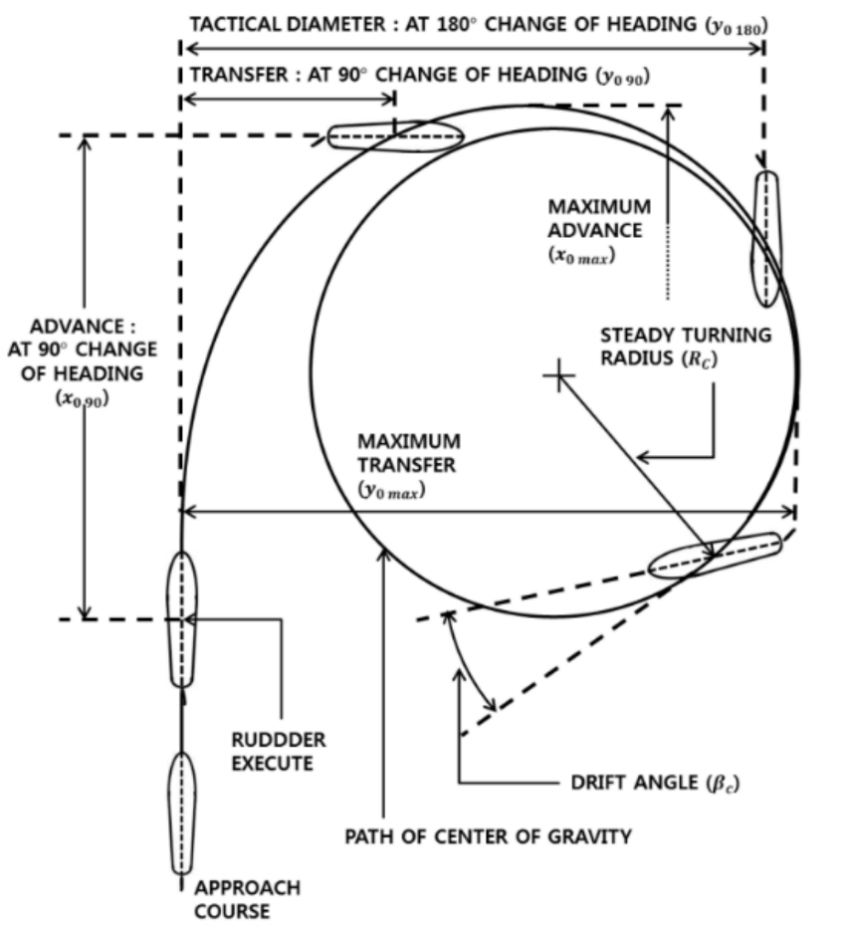
\includegraphics[width=4.70017in,height=5.14081in]{media/image4.png}
\caption{Sea trial designed for measuring the vessel's turning radius \cite{ref13}}\label{fig:image4}
\end{figure}

The information collected during automated sea trials gives vessel designers and engineers a good overview, which in turn is a great help when designing more capable vessels and developing existing watercraft.
